%use lualatex/xelatex to compile this
\documentclass{scrartcl}
\usepackage{polyglossia}
\setdefaultlanguage{english}

\usepackage{marvosym}% für den Smiley :-)
\def\contradiction{\quad\text{\Large\Lightning}}
\usepackage{graphicx}
\usepackage{float}
\usepackage{listings}
\usepackage{color}
\usepackage{enumerate}

\lstset{%
  literate={ö}{{\"o}}1%
           {ä}{{\"a}}1%
           {ü}{{\"u}}1%
           {Ö}{{\"O}}1%
           {Ä}{{\"A}}1%
           {Ü}{{\"U}}1%
           {ß}{{\ss}}1%
}

\definecolor{bggray}{rgb}{0.90,0.90,0.90}
\definecolor{dkgreen}{rgb}{0.00,0.50,0.00}
\definecolor{mauve}{rgb}{0.50,0.00,0.30}
\definecolor{darkGray}{rgb}{0.40,0.40,0.40}
\lstset{%
  language=C++,                   % the language of the code
  basicstyle=\small\ttfamily,
  numbers=none,                   % where to put the line-numbers
  backgroundcolor=\color{bggray}, % choose the background color. You must add \usepackage{color}
  showspaces=false,               % show spaces adding particular underscores
  showstringspaces=false,         % underline spaces within strings
  showtabs=false,                 % show tabs within strings adding particular underscores
  frame=single,                   % adds a frame around the code
  tabsize=4,                      % sets default tabsize to 2 spaces
  breaklines=true,                % sets automatic line breaking
  breakatwhitespace=true,         % sets if automatic breaks should only happen at whitespace
  title=\lstname,                 % show the filename of files included with \lstinputlisting;
                                  % also try caption instead of title
  keywordstyle=\color{blue},      % keyword style
  commentstyle=\color{dkgreen},   % comment style
  stringstyle=\color{mauve},      % string literal style
  escapeinside={\%*}{*)},         % if you want to add a comment within your code
}

\usepackage{amsmath,amsfonts,amsthm,amssymb,bbm,dsfont,mathrsfs}
\delimitershortfall=-3pt %makes parentheses grow larger automagically

\DeclareMathOperator*{\argmin}{argmin}
\DeclareMathOperator{\argmax}{argmax}
\DeclareMathOperator*{\cupdot}{\stackrel{{}_\bullet}{\cup}}
\DeclareMathOperator*{\bigcupdot}{\stackrel{{}_\bullet}{\bigcup}}
\def\LHS{&\phantom{{}=}} % First line of align environment with no relation symbol should still be align with the other lines. This is a dirty fix.
\usepackage{txfonts}

%Komma und Punktabstände anpassen:
%\mathcode`,="013B %nervt, außerdem braucht niemand Kommazahlen.
%\mathcode`.="613A

\author{Stefan Walzer}

%MENGEN Symbole
\newcommand{\R}{\ensuremath{\mathbb R}}
\newcommand{\N}{\ensuremath{\mathbb N}}
\newcommand{\Z}{\ensuremath{\mathbb Z}}
\newcommand{\Q}{\ensuremath{\mathbb Q}}
\newcommand{\C}{\ensuremath{\mathbb C}}
\newcommand{\K}{\ensuremath{\mathbb K}}

%Quantoren
\newcommand{\E}{\ensuremath{\exists}}
\newcommand{\A}{\ensuremath{\forall}}

%Pfeile
\newcommand{\LA}{\ensuremath{\Leftarrow}}
\newcommand{\RA}{\ensuremath{\Rightarrow}}
\newcommand{\la}{\ensuremath{\leftarrow}}
\newcommand{\ra}{\ensuremath{\rightarrow}}
\newcommand{\LRA}{\ensuremath{\Leftrightarrow}}
\newcommand{\lra}{\ensuremath{\leftrightarrow}}
\newcommand{\LLRA}{\ensuremath{\Longleftrightarrow}}
\newcommand{\llra}{\ensuremath{\longleftrightarrow}}

%spitze Klammern
\newcommand{\lan}{\ensuremath{\langle}}
\newcommand{\ran}{\ensuremath{\rangle}}


%Symbole
\newcommand{\veps}{\ensuremath{\varepsilon}}

%Verknüpfungen
\newcommand{\AND}{\wedge} %und
\newcommand{\OR}{\vee} %oder
\newcommand{\UN}{\cup} %union
\newcommand{\IS}{\cap} %intersection

%sonstiges
\def\abs#1{\left|#1\right|}
\def\norm#1{\lVert#1\rVert}
\def\floor#1{\left\lfloor#1\right\rfloor}
\def\ceil#1{\left\lceil#1\right\rceil}
\def\enquote#1{\glqq #1 \grqq}

\def\powset#1{\mathscr{P}\left(#1\right)}
\def\set#1{\left\{#1\right\}}
\def\setgen#1#2{\left\{#1\;\middle|\;#2\right\}}

%vector
\newcommand{\vect}[1]{\begin{pmatrix}#1\end{pmatrix}}
\newcommand{\svect}[1]{\scalebox{0.7}{$\begin{pmatrix}#1\end{pmatrix}$}}

%Fonts:

\setmainfont[Ligatures=TeX,SmallCapsFont={Latin Modern Roman Caps}]{Georgia}
\setsansfont{Segoe UI}
\setmonofont{Consolas}
\usepackage{unicode-math}
\setmathfont{xits-math.otf}

\usepackage{newunicodechar}
\usepackage{tikz}
\newunicodechar{Ø}{\emptyset}
\tikzset{node distance=3.5cm, auto}

\begin{document}
    \section*{Excercise 2}
    
    \begin{description}
        \item[a)] I show that $(C_1 × C_2)^B \cong C_1^B × C_2^B$. Consider the following diagram:
    \begin{figure}[H]
        \centering
    \begin{tikzpicture}
      \node  (C) {$(C_1 × C_2)^B × B$} ;
      \node  (P) [below of=C] {$C_1 × C_2$};
      \node  (C1) [left of=P] {$C_1$};
      \node  (C2) [right of=P] {$C_2$};
      \node  (P1) [left of=C] {$C_1^B × B$};
      \node  (P2) [right of=C] {$C_2^B × B$};
      \node  (CU) [above of=C] {$C_1^B × C_2^B × B$};
      
      \draw[->] (C) to node {$ε$} (P);
      \draw[->] (P) to node {$π_1$} (C1);
      \draw[->] (P) to node {$π_2$} (C2);
      \draw[->] (P1) to node {$ε$} (C1);
      \draw[->] (P2) to node {$ε$} (C2);
      \draw[->] (CU) to node {$π_1 × 1_B$} (P1);
      \draw[->] (CU) to node {$π_2 × 1_B$} (P2);
      \draw[->,dotted] (C) to node {$\bar{f_1} × 1_B$} (P1);
      \draw[->,dotted] (C) to node {$\bar{f_2} × 1_B$} (P2);
      \draw[<->,dotted] (CU) to node {$\star$} (C);
    \end{tikzpicture}
    \end{figure}
        The solid lines are the evaluation functions for the exponentials (note: the three $ε$ are all different) and the canonical projections for products.
        
        By the universal property of the exponential, there is exactly one $\bar{f_1}$ and $\bar{f_2}$ such that $\bar{f_1} × 1_B$ and $\bar{f_2} × 1_B$ make the diagram commute at the dashed lines ($f_1$ is $π_1 \circ ε$ here). Now, by the universal property of the product it is exactly $\bar{f_1} × \bar{f_2} × 1_B$ in the upwards direction at $\star$ that makes the diagram commute (requiring identity on the $B$ part).
        
        For the other direction note that by the universal property of the product there is exactly one morphism from $C_1^B × C_2^B × B$ to $C_1 × C_2$ that makes the diagram commute and this gives us (by the universal property of the exponential) the unique morphism $f : C_1^B × C_2^B → (C_1 × C_2)^B$ such that $f × 1_B$ in the downward dirction of $\star$ that makes the diagram commute.
        
        Together we have found two unique morphisms from at $\star$ that don't touch the $B$ part. Those must therefore be isomorphisms.
        
        \item[b)] Consider the following diagram:\begin{figure}[H]
        \centering
    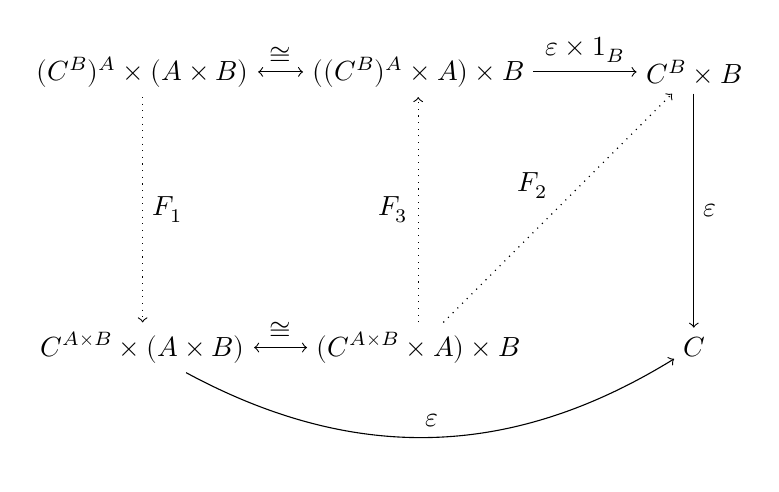
\begin{tikzpicture}
      \node  (O1) {$(C^B)^A × (A × B)$} ;
      \node  (O2) [right of=O1] {$((C^B)^A × A) × B$};
      \node  (O3) [right of=O2] {$C^B × B$};
      \node  (U1) [below of=O1] {$C^{A ×B} × (A × B)$};
      \node  (U2) [right of=U1] {$(C^{A ×B} × A) × B$};
      \node  (U3) [right of=U2] {$C$};
      
      \draw[<->] (O1) to node {$\cong$} (O2);
      \draw[<->] (U1) to node {$\cong$} (U2);
      \draw[->] (O2) to node {$ε × 1_B$} (O3);
      \draw[bend right,->] (U1) to node {$ε$} (U3);
      \draw[->] (O3) to node {$ε$} (U3);
      \draw[->,dotted] (O1) to node {$F_1$} (U1);
      \draw[->,dotted] (U2) to node {$F_2$} (O3);
      \draw[->,dotted] (U2) to node {$F_3$} (O2);
    \end{tikzpicture}
    \end{figure}
        It uses the cannonical isomorphisms (using associativity of products) and the respective evaluation functions of exponentials.
        
        We can construct the following morphisms uniquely:
        
        \begin{itemize}
            \item $f_1$ such that $F_1 = f_1 × 1_{A × B}$ makes the diagram commute (property of exponentials).
            \item $f_2$ such that $F_2 = f_2 × 1_B$ makes the diagram commute (property of exponentials).
            \item $f_3$ such that $F_3 = f_3 × 1_A × 1_B$ makes the diagram commute (property of exponentials).
        \end{itemize}
        
        We have now constructed $f_1 : (C^B)^A → C^{A × B}$ and $f_3$ in the other direction uniquely. These two functions must therefore be isomorphisms.
    \end{description}
    
    \section*{Excercise 3}
    
    We know that the transpose of a function is unique, i.e. if we find a function fullfilling the property of the transpose, we know that it must be the transpose. That being said:
    
    \begin{itemize}
        \item The transpose of $ε$ is $1_{B^A}$, since the following commutes:
        
        \begin{figure}[H]\centering\begin{tikzpicture}
      \node  (O1) {$B^A × A$} ;
      \node  (O2) [right of=O1] {$B$};
      \node  (U1) [below of=O1] {$B^A × A$};
      
      \draw[->] (O1) to node {$ε$} (O2);
      \draw[->] (U1) to node {$1_{B^A} × 1_A$} (O1);
      \draw[->] (U1) to node {$ε$} (O2);
    \end{tikzpicture}
    \end{figure}
    \item The transpose of $1_{A × B}$ in {\bf Sets} is:
    \[ f : a \mapsto (f_a : b \mapsto (a,b)) \] because this makes the diagram commute:
    \begin{figure}[H]\centering\begin{tikzpicture}
      \node  (O1) {$(A × B)^B × B$} ;
      \node  (O2) [right of=O1] {$A × B$};
      \node  (U1) [below of=O1] {$A × B$};
      
      \draw[->] (O1) to node {$ε$} (O2);
      \draw[->] (U1) to node {$f × 1_B$} (O1);
      \draw[->] (U1) to node {$1_{A × B}$} (O2);
    \end{tikzpicture}
    \end{figure}
    \item The transpose of $ε \circ τ$ in {\bf Sets} is:
    \[ f : a \mapsto (i_a : g \mapsto g(a)) \] (i.e. $f$ is the function that maps $a$ to the function $i_a$ that inserts $a$ into whatever function it gets as its paramter) because this makes the diagram commute:
    \begin{figure}[H]\centering\begin{tikzpicture}
      \node  (O1) {$B^{(B^A)} × B^A$} ;
      \node  (O2) [right of=O1] {$B$};
      \node  (U1) [below of=O1] {$A × B^A$};
      \node  (U2) [right of=U1] {$B^A × A$};
      
      \draw[->] (O1) to node {$ε$} (O2);
      \draw[->] (U1) to node {$f × 1_{B^A}$} (O1);
      \draw[->] (U1) to node {$τ$} (U2);
      \draw[->] (U2) to node {$ε$} (O2);
    \end{tikzpicture}
    \end{figure}
    \end{itemize}
\end{document}